\newpage
\section{Printaufbau}
\label{sec:Printaufbau}

In Abbildung \ref{fig:Print_3D} ist der Aufbau des entstandenen Prints zu sehen. Auf diesem sind die in Abbildung  \ref{fig:Blockschaltbild_Partymixer} gezeigte Blöcke wieder zu erkennen. In Tabelle \ref{tab:table} und Abbildung \ref{fig:figure} ist zusätzlich ein Layer-Detail des Herstellers und dessen Spezifikationen zum Print zu sehen. Das Schema zum Print befindet sich im Anhang Kapitel \ref{Appendix:Schema_Print}.

\begin{figure}[H]
	\centering
	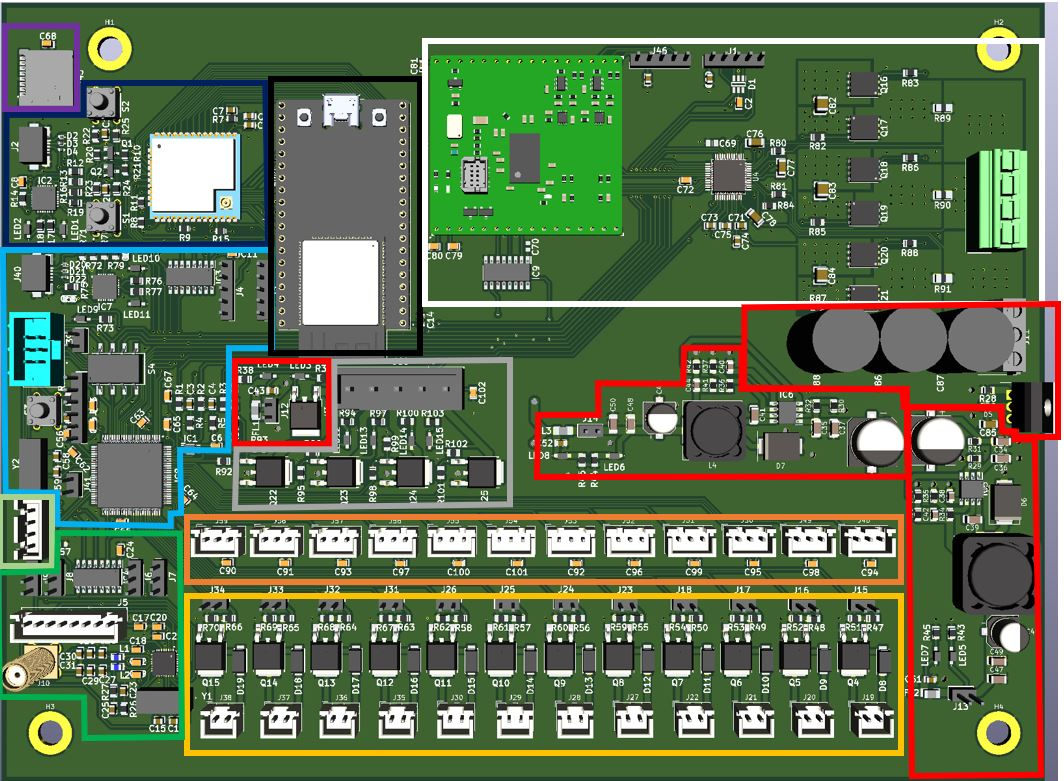
\includegraphics[width=0.9\textwidth]{graphics/Printteile}
	\caption{Aufbau des Prints als Modell}
	\label{fig:Print_3D}
\end{figure} 

\begin{table}[H]%
\centering
\parbox{0.5\textwidth}{
\begin{footnotesize}
\begin{tabular}{|l|ll|}
\hline
\multicolumn{3}{|c|}{\textbf{Technische Details Print}}\\
\hline
Dimensionen & 222mm x 166mm & ($\pm$ 0.2mm)\\
\hline
PCB Dicke & 1.6mm & ($\pm$ 10\%)\\
\hline
Material & FR-4 & (Tg 130-140C)\\
\hline
Oberfläche & HASL & (with lead)\\
\hline
Anzahl Layers & 4 & \\
\hline
Top / Bottom & 1oz & (35$\mu$m)\\
\hline
Layer 2 / 3 & 0.5oz & (17$\mu$m)\\
\hline
\end{tabular}
\end{footnotesize}
\caption{Spezifikationen der Platine \cite{jlcpcb_jlcpcb_2020}}
\label{tab:table}
}
\qquad
\begin{minipage}[c]{0.43\textwidth}%
\centering
\begin{figure}[H]
    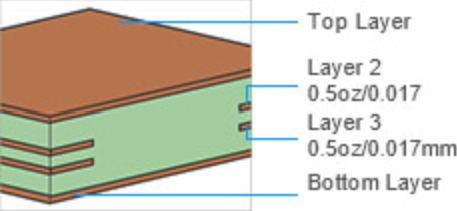
\includegraphics[width=1\textwidth]{graphics/Print_Layers}
\caption{Querschnitt der Platine \cite{jlcpcb_jlcpcb_2020}}
\label{fig:figure}
\end{figure}
\end{minipage}
\end{table}

Der Print ist grundsätzlich in zwei Gruppen unterteilt. Der rechte Teil des Prints beinhaltet den Leistungsteil und auf der linken Seite des Prints ist der Logigteil zu finden. In Abbildung \ref{fig:Print_3D} sind die einzelnen Teile auf dem Print in Farben unterteilt. Die Aufgabenbereiche und die Funktionsweise der einzelnen Teile werden in Kapitel \ref{sec:Teilsysteme} behandelt.\\

\textcolor{red}{\textbf{\underline{Speisungen:}}}
In den rot markierten Bereichen sind die Speisungsteile zu sehen, wobei sich auf der rechten Seite des Prints die Eingangskondensatoren mit Verpolschutz, die 12V-Speisung und die 5V-Speisung befinden. Das 48V-Netzteil ist gemäss Blockschaltbild \ref{subsec:Blockschaldbild} extern angebracht. Im Logikteil des Prints auf der linken Seite ist die 3.3V-Speisung zu finden.

\textcolor{ProcessBlue}{\textbf{\underline{Mikrocontroller:}}}
Im hellblau markierten Bereich auf der linken Seite des Prints befindet sich das Herzstück der Elektronik. Der Mikrocontroller mit der dazugehörigen Programmierschnittstelle, welche einen Micro-USB Anschluss zu Programmierzwecken beinhaltet.

\textcolor{Goldenrod}{\textbf{\underline{Pumpenansteuerung:}}}
Auf der unteren Seite des Prints sind im gelben Bereich die Anschlüsse der Pumpen zu finden, welche die Flüssigkeiten befördern. Dazu gehört jeweils eine kleine Leistungsansteuerung mittels Logik-MOSFET und Freilaufdiode. 

\textcolor{orange}{\textbf{\underline{Durchflussmessgeräte:}}} Über der Pumpenansteuerung befinden sich im orange markierten Bereich die Anschlüsse der Durchflussmessgeräte, welche auch die Speisung der Durchflussmessgeräte und einen Entstörkondensator beherbergen.

\textcolor{gray}{\textbf{\underline{Maschinenbeleuchtung:}}}
Um die Maschine mit einem Showeffekt auszustatten wurde eine Lichtansteuerung eines RGBW-LED-Streifen implementiert gemäss Kapitel \ref{subsec:Blockschaldbild}. Diese ist im grau markierten Bereich zu finden und beinhaltet einen Anschluss, sowie vier Logik-MOSFET's zur Ansteuerung.

\textcolor{blue}{\textbf{\underline{Wireless- /Bluetoothmodul:}}}
Um mit externen Gerätschaften kommunizieren zu können, befindet sich im Dunkelblau markierten Bereich das Wireless- / Bluetoothmodul. Auch dieses beinhaltet neben dem eigentlichen Modul eine dazugehörige Programmierschnittstelle gemäss Blockschaldbild \ref{fig:Blockschaltbild_Partymixer}.

\textcolor{violet}{\textbf{\underline{SD-Karte:}}}
Der microSD-Kartenslot befindet sich links oben im Violett markierten Bereich.


\textcolor{lightgray}{\textbf{\underline{Motoransteuerung:}}}
Die Motorenansteuerung ist im weissen Teil des Print's zu finden. Sie hat einen grossen Teil des Prints in Beschlag genommen und ist von links nach rechts in drei Teile unterteilt. Als Erstes der FOC-Treiber, gefolgt vom Gate-Treiber und der H-Brücke mit dem Anschluss des Motor's. Dieser Teil ist jedoch bei der fertigen Maschine durch externe Elektronik ersetzt worden. 

\textcolor{LimeGreen}{\textbf{\underline{Display:}}}
Das Display benötigt keine grosse Ansteuerungslogik und besteht aus diesem Grund auch nur aus einem einzelnen Stecker. Dieser befindet sich im Bereich des Mikrocontrollers, im hellgrün markierten Bereich.

\textcolor{black}{\textbf{\underline{Wireless- /Bluetoothmodul 2:}}}
Aus Sicherheitsgründen wurde für den Fall, dass Probleme bei der Inbetriebnahme auftauchen, ein Steckplatz für ein Evaluationsboard des Wireless- / Bluetoothmoduls implementiert. Dieses wird jedoch nicht verwendet. Somit generiert dies neue Möglichkeiten für weitere Anschlüsse am Wireless- / Bluetoothmodul im Dunkelblauen Teil. An diesen Anschlüssen befindet sich nun das RFID Evaluationsboard sowie die SPI-Leitungen vom Mikrocontroller zum FOC-Treiber. 

\textcolor{ForestGreen}{\textbf{\underline{RFID-Modul:}}}
Für den Fall, dass noch genügend Zeit übrigbleiben sollte, wurde ein eigenes RFID-Board gelayoutet. Diese ist im dunkelgrünen Bereich zu sehen. Dieses wird jedoch in diesem Projekt nicht verwendet, da sich das RFID-Modul nun im schwarz markierten Bereich als Evaluationsboard befindet. 

Auf dem Print mussten im Laufe des Projektes kleinere Anpassungen vorgenommen werden. Dies gehört zum Entwicklungsprozess dazu. Somit mussten zum Beispiel Leitungen aufgetrennt werden, neue Leitungen geschaffen oder sogar neue Baugruppen implementiert werden. Die Änderungen sind im Schema Rot gekennzeichnet.